% siminos/presentations/kittens/reversal.tex        pdflatex reversal; biber reversal
% $Author: predrag $ $Date: 2021-12-06 11:25:30 -0500 (Mon, 06 Dec 2021) $

% remember to update \date{December 6, 2021}

                        \newif\ifboyscout\boyscouttrue          %% comments     %%
                        \newif\ifsubmission\submissionfalse     %% internal     %%
                        \newif\ifblog\blogfalse %% section shared with blogCats %%

\input ../../inputs/layoutBeamer
\usepackage[font=scriptsize, labelfont=bf]{caption}
\usepackage[
    backend=biber,  %bibtex,
    sorting=nyt,
    %refsection=chapter,
    %citereset=chapter,
    style=numeric, %alphabetic, % %style=authoryear,
    natbib=true,
    style=phys, % aps
    biblabel= brackets, % superscript, %
    articletitle=false, % true,  % false, % aps
    %chaptertitle=true,  % aip;  % false, % aps
    pageranges = true , % aip: the full range
             % = false, % aps: only the first page being printed
    sortlocale=en_US,
    firstinits=true,
    url=false, %true,  %
    doi=false, %true,
    eprint=false
]{biblatex}
\addbibresource{../../bibtex/siminos.bib}
\setbeamerfont{footnote}{size=\tiny}
%\input ../../inputs/def % no edits, always from dasbuch/book/inputs
\input defsKittens
\input ../../inputs/defsBeamer

%      \renewcommand{\statesp}{phase space}
\renewcommand{\statesp}{state space}
\renewcommand{\Statesp}{State space}
\renewcommand{\Refl}{\ensuremath{\sigma}}             % in DasBuch
%\renewcommand{\Refl}{\ensuremath{{s}}} % Dihedral wiki convention
\renewcommand{\shift}{\ensuremath{r}}
\renewcommand{\hopMat}{\shift} % Aug 2021 experimental, eventually eliminate
%\newcommand{\hopMat}{\mathbf{\sigma}} % Dec 2012 experimental
\renewcommand{\ssp}{\ensuremath{\phi}}             % lattice site field
%\renewcommand{\Xx}{\ensuremath{\mathsf{\Phi}}}      % kittens lattice field
%   there is no font for \mathsf{\Phi}}?
\renewcommand{\Ssym}[1]{{\ensuremath{m_{#1}}}}    % Boris


\begin{document}
\title{
{\huge chaotic field theory %\catlatt}
    \\
        time reversal}
%{back to "amazing! I did not understand a single word!"}
}
\author{P. Cvitanovi\'c}
\author[Cvitanovi\'c]
{
  \textcolor{green!50!black}{
  {
Predrag~Cvitanovi\'c
   and
Han Liang
%   \\
%  Matt Gudorf,
  }	%\inst{1}
  }
}
\institute
{               Georgia Tech     \\
                {\scriptsize
 ChaosBook.org/overheads/spatiotemporal \\
 $\to$ Chaotic field theory slides    }
 }
\date{December 6, 2021}

\begin{frame}
  \titlepage
\end{frame} %%%%%%%%%%%%%%%%%%%%%%%%%%%%%%%%%%%%%%%%%%%%%%

%\begin{frame}{Nordita Quantum Chaos Symposium, 25 Nov 1988}
%\begin{center}
%\hfill\includegraphics[width=0.95\textheight]{IMG_3109}
%\end{center}
%
%\begin{bartlett}
%     Amazing! I did not understand a single word.
%\bauthor{Fritz Haake}
%\end{bartlett}
%\end{frame} %%%%%%%%%%%%%%%%%%%%%%%%%%%%%%%%%%%%%%%%%%%%%%

\begin{frame}{chaotic / turbulent field theory?}
herding cats audience reviews:%
\footnote{the limiting speed for transfer of quantum-chaotic information is 1 Prozen.}
\begin{center}
  \begin{minipage}[b]{0.42\textwidth}

\bigskip
Arnd B\"acker: \\ {\footnotesize "even faster than Toma\v{z} Prosen"}

\bigskip
Martina Hentschel: \\ {\footnotesize "Amazing :)"}

\bigskip
Arnd B\"acker: \\ {\footnotesize "... maybe  I even understood \\ a single word..."}
  \end{minipage}
\qquad\quad
  \begin{minipage}[b]{0.46\textwidth}\hfill

\includegraphics[width=1.00\textwidth]{DawnBishopCats}
  \end{minipage}
\end{center}
\end{frame} %%%%%%%%%%%%%%%%%%%%%%%%%%%%%%%%%%%%%%%%%%%%%%


%\section[what this talk is about]
% {what this talk is about}
%
%\begin{frame}{overview}
%\begin{enumerate}
%              \item {\Large
%what this is about
%                  }\textcolor{gray}{\small
%%\\{\scriptsize \em
%%  (to skip the motivational blah blah: go to part \textcolor{red}{\ref{spacetimeFT}})
%%  }
%              \item
%chaos - a short course
%              \item
%\templatt
%              \item
%\catlatt
%              \item
%space is time
%              \item
%bye bye, dynamics
%                    }
%            \end{enumerate}
%\end{frame} %%%%%%%%%%%%%%%%%%%%%%%%%%%%%%%%%%%%%%%%%%%%%%


\section[time reversal]
 {time reversal}

\begin{frame}{Euclidean lattice field theory}
    \begin{block}{scalar \emph{field} $\ssp(x)$}
 evaluated on lattice points
%\bigskip

\begin{center}
            \begin{minipage}[c]{0.32\textwidth}\begin{center}
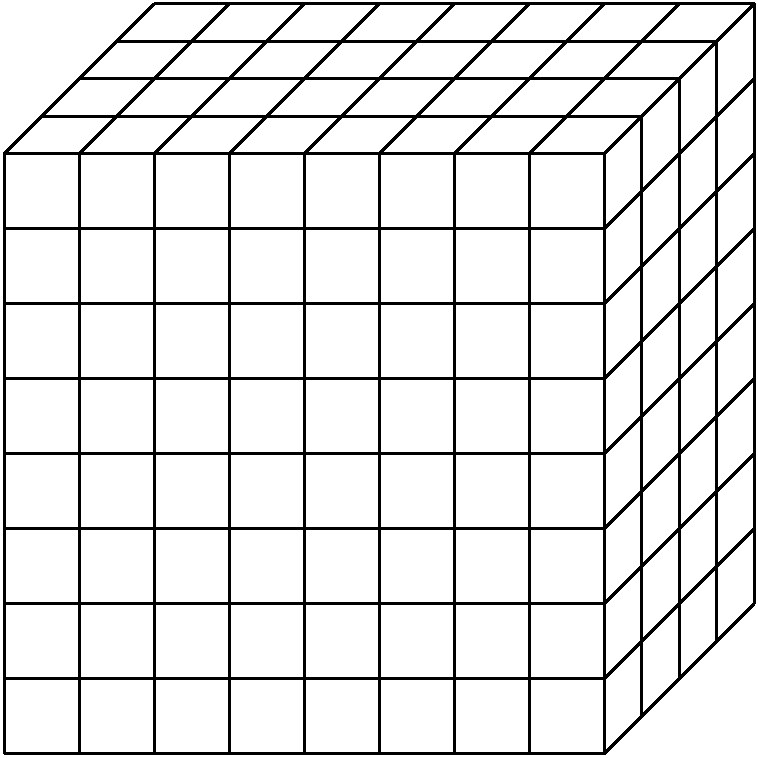
\includegraphics[width=0.95\textwidth]{MunWal00lattice}
            \end{center}
% 3$d$ lattice
% \label{fig:MunWal00lattice}
            \end{minipage}
            \hspace{2ex}
            \begin{minipage}[c]{0.46\textwidth}
$\ssp_z
=
\ssp(x)$
\\
$
x = a\,z= \mbox{lattice point}$
\\
$
z \in \integers^d %/\speriod{}^d
$
%\ee{LattField}
            \end{minipage}
\end{center}
a periodic point per each unit cell
    \end{block}
\footfullcite{MunWal00}
\end{frame} %%%%%%%%%%%%%%%%%%%%%%%%%%%%%%%%%%%%%%%%%%%%%%

\begin{frame}{example : discretization of a $1d$ field}
    \begin{block}{scalar \emph{field} $\ssp(x)$ evaluated on lattice points}

\begin{center}
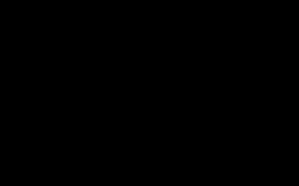
\includegraphics[width=0.55\textwidth]{LC21FieldConfig}

\bigskip
            \begin{minipage}[c]{0.42\textwidth}
periodic field $\ssp(\zeit)$
\\
is a function of
\\
continuous coordinate $\zeit$
            \end{minipage}
            \hspace{2ex}
            \begin{minipage}[c]{0.42\textwidth}
corresponding discretized period-$5$ {\lattstate}
\\
$\Xx=\cycle{\ssp_0 \ssp_1 \ssp_2 \ssp_3 \ssp_4}$,
            \end{minipage}
\end{center}
    \end{block}
Horizontal: $\zeit$ coordinate, lattice sites marked by
\\
dots, labelled by $\zeit\in\integers$

\medskip
the value of the discretized field $\ssp_\zeit\in\reals$ is plotted as
\\
a bar centred at lattice site $\zeit$
\end{frame} %%%%%%%%%%%%%%%%%%%%%%%%%%%%%%%%%%%%%%%%%%%%%%

\begin{frame}{Bravais cell lattice tiling}
 write a periodic field over \cl{}-sites Bravais cell as \\
the {\color{blue}{\lattstate}} and
the {\color{blue}symbol \brick} (sources)
\beq
{\Xx} % = \{\ssp_j\}
             = (\ssp_{\zeit+1},\cdots,\ssp_{\zeit+\cl{}})
\,,\quad
{\Mm} % = \{\Ssym{j}\}
             = (\Ssym{{\zeit+1}},\cdots,\Ssym{{\zeit+\cl{}}})
\ee{pathBern}
\begin{center}
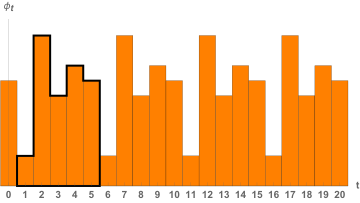
\includegraphics[width=0.85\textheight]{HL1dLatticeStateBar1}
\end{center}

`$\Mm$' for `marching orders' ~~:~~ come here, then go there, $\cdots$
\end{frame} %%%%%%%%%%%%%%%%%%%%%%%%%%%%%%%%%%%%%%%%%%%%%%

\begin{frame}{field theory is defined by its action}
    \begin{block}{field theory}
\textcolor{blue}{field configuration} \Xx\ occurs with probability
\[
p(\Xx)\,=\, \frac{1}{Z}\,e^{-S[\Xx]}
\,,\qquad Z=Z[0]
\] % ee{ProbConf}
\textcolor{blue}{partition function} $=$ sum over all
configurations
\beq
Z[\source]	% = e^{W[\source]}
    \,=\, \int [d\ssp]\,e^{-S[\Xx] + \Xx \cdot \source}
    \,,\qquad
\left[ d\ssp\right] = \prod_{z}^{\lattice} \frac{d\ssp_z}{\sqrt{2 \pi}}
\label{n-pt-corr}
\eeq

\textcolor{blue}{`source'} $\source$
    \end{block}
\end{frame} %%%%%%%%%%%%%%%%%%%%%%%%%%%%%%%%%%%%%%%%%%%%%%

\begin{frame}{example : Euclidean {$\phi^4$} theory}
    \begin{block}{continuum action}
\bea
S &=&
\int dx^d \left\{ \frac{1}{2} \sum_{i =1}^d
(\partial_{\mu}\ssp(x))^2 + \frac{\mu^2}{2}\ssp(x)^2 + \frac{g}{4!}\ssp(x)^4
\right\}
\eea
    \end{block}

    \begin{block}{lattice action}
\bea
S[\Xx] &=&
\sum_{z,z'} \frac{1}{2}\left\{
\ssp_z\left(-\Box + \mu^2\right)_{zz'}\ssp_{z'}
\right\}
 + \sum_{z}\frac{g}{4!}\ssp_z^4
\,.
%\label{MunWal00freeAct}
\eea
    \end{block}

in `lattice units' : \(a=1\)
\end{frame} %%%%%%%%%%%%%%%%%%%%%%%%%%%%%%%%%%%%%%%%%%%%%%

\begin{frame}{QFT path integrals : semi-classical WKB quantization}
  \begin{columns}
  \column{0.42\textwidth}
\begin{block}{WKB backbone}
\textcolor{blue}{classical field theory}
\\
extremal condition $\to$ eqs
\beq
\frac{\delta{S[\Xx]}}{\delta\ssp_z~}=\Ssym{z}
\ee{LC21eqMotion}
classical solution \Xx\ satisfies
the local extremal condition on every lattice site
\end{block}
  \column{0.50\textwidth}
\begin{block}{a fractal set of saddles}
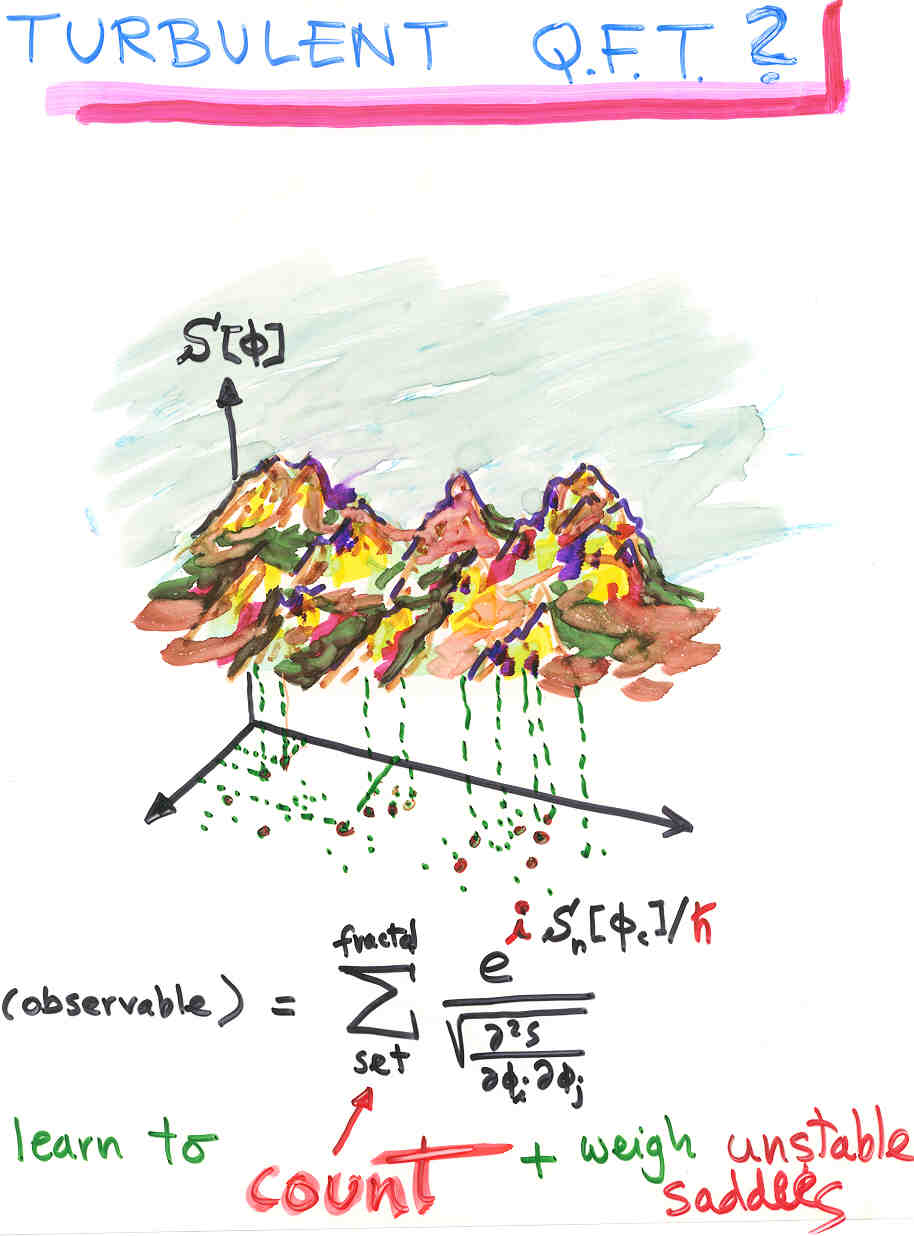
\includegraphics[width=1.00\textwidth,clip=true]{pde2}%
\end{block}
  \end{columns}
\end{frame}

\begin{frame}{think globally, act locally}
    \begin{center}
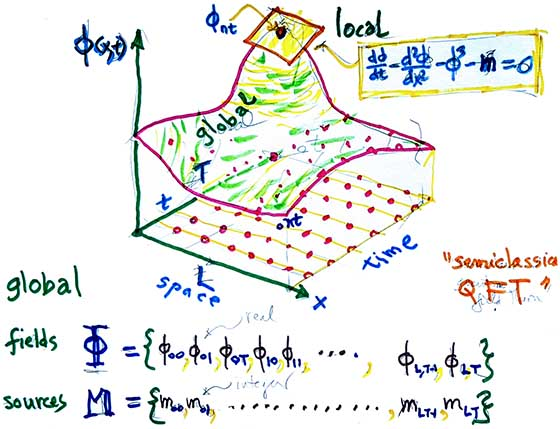
\includegraphics[width=0.85\textwidth]{globalLocal}
    \end{center}
for each symbol array \Mm, a periodic {\lattstate} $\Xx_\Mm$
\end{frame} %%%%%%%%%%%%%%%%%%%%%%%%%%%%%%%%%%%%%%%%%%%%%%

\begin{frame}{Laplacian discretization}
discrete lattice
\begin{block}{Laplacian in $1$ dimension}
\[
\ssp_{\zeit+1} - 2\ssp_{\zeit} + \ssp_{\zeit-1}
     =
\Box\,\ssp_{\zeit}
\]
\end{block}
\medskip

so have an (anti)oscillator chain, known as
\begin{block}{$d=1$ Klein-Gordon (or damped Poisson) equation}
\[
 (-\Box + {\mu}^2)\,\ssp_{\zeit} = \m_t
\,, \qquad
{\mu}^2= s-2
\] %\ee{LinearConn}
\end{block}
\end{frame} %%%%%%%%%%%%%%%%%%%%%%%%%%%%%%%%%%%%%%%%%%%%%%

\begin{frame}{examples : 1$d$ lattice field theories}

{\color{orange}spatio}temporal lattice field theory
\bea
- \ssp_{\zeit+1}  + V'[\ssp_{\zeit}] - \ssp_{\zeit-1}
    &=&
\Ssym{\zeit}
%\,,\qquad  \ssp_{\zeit} \in [0,1)
%\label{LC21:1dTempFT}
\eea

{\color{orange}spatio}temporal  Bernoulli
\bea
- \ssp_{\zeit+1} + {s}\,\ssp_{\zeit}
    \qquad\quad\;
    &=&
\Ssym{\zeit}
%\,,\qquad  \ssp_{\zeit} \in [0,1)\,,
%\label{LC21:1dBernLatt}    % labelled {1stepDiffEq} elsewhere
\eea

{\color{orange}spatio}{\templatt}
\bea
- \ssp_{\zeit+1}  +  \,{s}\,\ssp_{\zeit} - \ssp_{\zeit-1}
    &=&
\Ssym{\zeit}
%\,,\qquad  \ssp_{\zeit} \in [0,1)
\eea %    \continue %\label{LC21:1dTemplatt}\\
{\color{orange}spatio}{\henlatt}
\bea
- \ssp_{\zeit+1} + {a}\,\ssp_{\zeit}^2 - \ssp_{\zeit-1}
    &=&
\Ssym{\zeit}
%\,,\qquad  \Ssym{\zeit}=2
\eea %    \continue %\label{LC21:1dHenlatt}\\
{\color{orange}spatio}temporal {$\phi^4$} theory
\bea
- \ssp_{\zeit+1} + \frac{g}{3!}\ssp_{\zeit}^3 - \ssp_{\zeit-1}
    &=&
\Ssym{\zeit}
%\,,
%\label{LC21:1dPhi4}
\eea
\end{frame} %%%%%%%%%%%%%%%%%%%%%%%%%%%%%%%%%%%%%%%%%%%%%%

\begin{frame}{herding cats in $d$ spacetime dimensions : `\catlatt'}
%\begin{center}
%\hfill
\includegraphics[width=0.55\textwidth]{spatiotempCat}
\hfill
\includegraphics[width=0.55\textwidth]{DawnBishopCats}
%\end{center}
\end{frame} %%%%%%%%%%%%%%%%%%%%%%%%%%%%%%%%%%%%%%%%%%%%%%

%\begin{frame}{}
%\begin{enumerate}
%              \item {\Large
%kicked rotor
%                  }\textcolor{gray}{\small
%              \item
%\catlatt
%              \item
%bye bye, dynamics
%                    }
%            \end{enumerate}
%\end{frame} %%%%%%%%%%%%%%%%%%%%%%%%%%%%%%%%%%%%%%%%%%%%%%

\begin{frame}{\catlatt\ : a strong coupling field theory}

%2020-09-05
%\subsection{Symmetries of the integer lattice}
%\label{s:lattSymm}
\begin{block}{\catlatt\ symmetries :}
translations $\circ$ time-reversal $\circ$ spatial reflections
\end{block}
point-group of the square lattice:
\\ rotations by $\pi/2$
\\ reflections across axes  and diagonals,
\[ %beq
\Dn{4} = \{
1, \shift, \shift^2, \shift^3,
\Refl, \Refl_{1},
\Refl_{2},\Refl_{3}
\}
\,.
\] %\ee{eq:C4v}
international crystallographic notation\footfullcite{Dresselhaus07},
\\
the square lattice space group $p4mm$.

\bigskip
{\color{red}not} a traditional \\
{\color{blue}spatially
weakly coupled} lattice model\footfullcite{BunSin88}
%\bigskip
%\vfill
\end{frame} %%%%%%%%%%%%%%%%%%%%%%%%%%%%%%%%%%%%%%%%%%%%%%

\begin{frame}{symmetries of a square lattice unit cell}
%%%%%%%%%%%%%%%%%%%%%%%%%%%%%%%%%%%%%%%%%%%%%%%%%%%%%%%%%%%%%%%%%%
% PC 2021-08-05:  from ChaosBook book/figs/D3.tex, D3.tex
\begin{center}
  \begin{minipage}[b]{0.39\textwidth}\begin{center}
  \setlength{\unitlength}{1.00\textwidth}
  \begin{picture}(1,0.94270725)%
    \setlength\tabcolsep{0pt}%
    \put(0,0){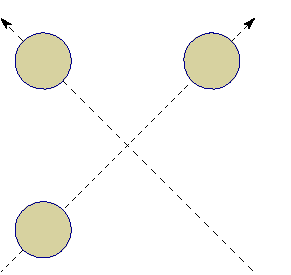
\includegraphics[width=\unitlength,page=1]{D4}}%
    \put(0.11589164,0.70318699){\color[rgb]{1,1,1}\makebox(0,0)[lt]{\smash{{\Large 2}}}}%
    \put(0.11465857,0.11853823){\color[rgb]{1,1,1}\makebox(0,0)[lt]{\smash{{\Large 3
    }}}}%
    \put(0,0){\includegraphics[width=\unitlength,page=2]{D4}}%
    \put(0.69662672,0.11848457){\color[rgb]{1,1,1}\makebox(0,0)[lt]{\smash{{\Large 0}}}}%
    \put(0.69785979,0.70163221){\color[rgb]{1,1,1}\makebox(0,0)[lt]{\smash{{\Large 1}}}}%
    \put(0.48887673,0.58974203){\color[rgb]{0.1372549,0.12156863,0.1254902}\makebox(0,0)[lt]{\smash{$\shift_1$}}}%
    \put(0,0){\includegraphics[width=\unitlength,page=3]{D4}}%
    \put(0.24073374,0.49925981){\color[rgb]{0.1372549,0.12156863,0.1254902}\makebox(0,0)[lt]{\smash{$\shift_2$}}}%
    \put(0.33991763,0.28480816){\color[rgb]{0.1372549,0.12156863,0.1254902}\makebox(0,0)[lt]{\smash{$\shift_3$}}}%
    \put(0.95378545,0.34914366){\color[rgb]{0.1372549,0.12156863,0.1254902}\makebox(0,0)[lt]{\smash{$\Refl_1$}}}%
    \put(0.87112523,0.73973783){\color[rgb]{0.1372549,0.12156863,0.1254902}\makebox(0,0)[lt]{\smash{$\Refl_2$}}}%
    \put(0.50562029,0.87631462){\color[rgb]{0.1372549,0.12156863,0.1254902}\makebox(0,0)[lt]{\smash{$\Refl_3$}}}%
    \put(0.11826698,0.87765494){\color[rgb]{0.1372549,0.12156863,0.1254902}\makebox(0,0)[lt]{\smash{$\Refl$}}}%
    \put(0,0){\includegraphics[width=\unitlength,page=4]{D4}}%
  \end{picture}
  \end{center} \end{minipage}
  \end{center}
%  \caption{\label{fig:D3D4}
% Dihedral group \Dn{3}: \Dn{4}:

4 rotations $\shift_j$, 4 shift-reflections
$\Refl_k$ of dihedral group
\[ %beq
\Dn{4} = \{
1, \shift, \shift^2, \shift^3,
\Refl, \Refl_{1},
\Refl_{2},\Refl_{3}
\}
\] %\ee{eq:C4v}
%even reflection axes dashed, odd reflections full line
overly the square onto itself.

They also tile it with  the $8$ copies $\pSRed_\ell$ of
\\
the {\color{blue}fundamental domain} (the shaded wedge)
\end{frame} %%%%%%%%%%%%%%%%%%%%%%%%%%%%%%%%%%%%%%%%%%%%%%

\begin{frame}{retreat to : 1$d$ lattice field theories}

{\color{orange}spatio}{\templatt}
\bea
- \ssp_{\zeit+1}  +  \,{s}\,\ssp_{\zeit} - \ssp_{\zeit-1}
    &=&
\Ssym{\zeit}
%\,,\qquad  \ssp_{\zeit} \in [0,1)
\eea %    \continue %\label{LC21:1dTemplatt}\\
{\color{orange}spatio}{\henlatt}
\bea
- \ssp_{\zeit+1} + {a}\,\ssp_{\zeit}^2 - \ssp_{\zeit-1}
    &=&
\Ssym{\zeit}
%\,,\qquad  \Ssym{\zeit}=2
\eea %    \continue %\label{LC21:1dHenlatt}\\
{\color{orange}spatio}temporal {$\phi^4$} theory
\bea
- \ssp_{\zeit+1} + \frac{g}{3!}\ssp_{\zeit}^3 - \ssp_{\zeit-1}
    &=&
\Ssym{\zeit}
%\,,
%\label{LC21:1dPhi4}
\eea
\end{frame} %%%%%%%%%%%%%%%%%%%%%%%%%%%%%%%%%%%%%%%%%%%%%%

\begin{frame} {in crystallography symmetries rule}
There are only two \HREF{https://en.wikipedia.org/wiki/Line_group}
{1\dmn\ space groups}  $\Group$:
\\
\textcolor{blue}{$p1$} \emph{infinite cyclic
group}  \Cn{\infty} of all lattice translations,
\beq
\Cn{\infty}
    =       \{
\cdots, \shift_{-2}, \shift_{-1},
        1,
        \shift_{1}, \shift_{2}, \shift_{3}, \cdots
             \}
\label{C_infty}
\eeq

\textcolor{blue}{$p1m$} \emph{infinite dihedral group} $\Dn{\infty}$  of all
translations and reflections\footfullcite{KiLePa03},
\beq
  \Dn{\infty} = \{
\cdots, \shift_{-2},\Refl_{-2}, \shift_{-1},\Refl_{-1},
        1,\Refl,
        \shift_{1},\Refl_{1}, \shift_{2},\Refl_{2}, \cdots
             \}
%\,.
\ee{LC21D_infty}
\textcolor{blue}{group multiplication}
$\LieEl_i\LieEl_j$
\beq
\begin{tabular}{c|cc}
%\Dn{\infty} &\shift_j        &\Refl_j\\\hline
            &$\shift_j$        &$\Refl_j$\\\hline
$\shift_i$  &$\shift_{i+j}$     &$\Refl_{j-i}$\\
$\Refl_i$   &$\Refl_{i+j}$     &$\shift_{j-i}$
\end{tabular}
\ee{eq:DinftyMultTab}
either adds up translations,
\\
or shifts and then reverses their direction
\end{frame} %%%%%%%%%%%%%%%%%%%%%%%%%%%%%%%%%%%%%%%%%%%%%%

\begin{frame} {Symmetries of 1\dmn\ Bravais sublattices}
\emph{Bravais cell} of \emph{period} \cl{} : given by vector
$\mathbf{a}$ of length \cl{}

\emph{Bravais  sublattice} generated by translations
\[
  \shift_{j}\to\shift_{j\mathbf{a}}
\]
symmetry : translation subgroup of $\Cn{\infty}$
\beq
H_{\mathbf{a}} = \{ \cdots, \shift_{-2 \mathbf{a}}, \shift_{-\mathbf{a}},
1, \shift_{\mathbf{a}}, \shift_{2 \mathbf{a}}, \cdots\}
\,,
\ee{H(n)subgroup}
and
% a tiling of the lattice $\integers$ by a generic
% {\lattstate} tile of length \cl{}
\[
  \shift_{j}\to\shift_{j\mathbf{a}}
\,,\qquad
    \Refl\to \Refl_{k}
  \quad
     0\leq{k}<\cl{}
\,,
\]
symmetry :  $\cl{}$ infinite dihedral subgroups of $\Dn{\infty}$
\beq
H_{\mathbf{a},k} = \{
\cdots, \shift_{-2 \mathbf{a}}, \Refl_{k}\shift_{-2 \mathbf{a}},
        \shift_{-\mathbf{a}}, \Refl_{k}\shift_{-\mathbf{a}},
        1,                    \Refl_{k},
        \shift_{\mathbf{a}},  \Refl_{k}\shift_{\mathbf{a}},
        \shift_{2\mathbf{a}},\Refl_{k}\shift_{2\mathbf{a}}, \cdots
             \}
\,,
\ee{H(n,k)subgroup}
{Bravais cell} of period \cl{},
\\
with reflection
across a symmetry point shifted $k$ 1/2 steps
\end{frame} %%%%%%%%%%%%%%%%%%%%%%%%%%%%%%%%%%%%%%%%%%%%%%

\begin{frame} {$\Dn{\infty}$ orbit of a generic {\lattstate}}
%%%%%%%%%%%%%%%%%%%%%%%%%%%%%%%%%%%%%%%%%%%%%%%%%%%%%
\begin{center}
  \begin{minipage}[b]{0.17\textwidth}\begin{center}
{(1)}~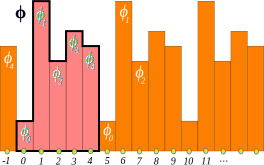
\includegraphics[width=\textwidth]{1dLatStatC_5_0}
\\
{($\shift_1$)}~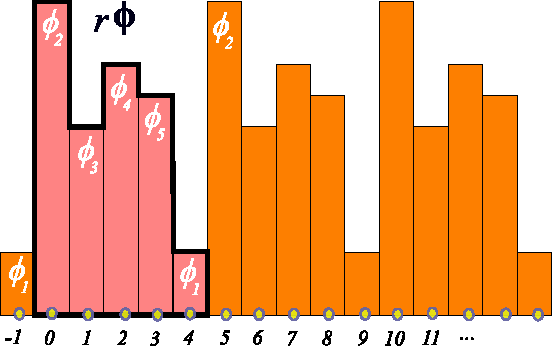
\includegraphics[width=\textwidth]{1dLatStatC_5_1}
\\
{($\shift_2$)}~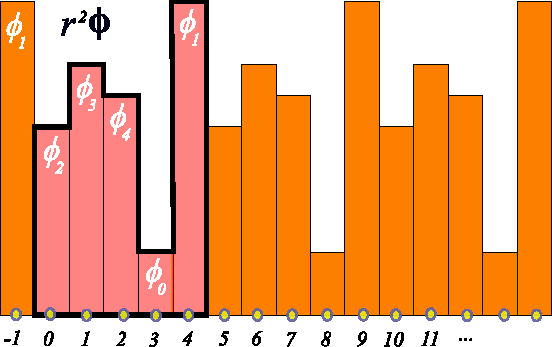
\includegraphics[width=\textwidth]{1dLatStatC_5_2}
\\
{($\shift_3$)}~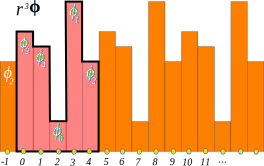
\includegraphics[width=\textwidth]{1dLatStatC_5_3}
\\
{($\shift_4$)}~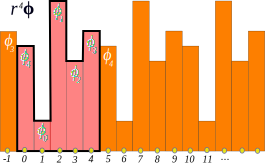
\includegraphics[width=\textwidth]{1dLatStatC_5_4}
  \end{center}\end{minipage}
\qquad\quad
  \begin{minipage}[b]{0.17\textwidth}\begin{center}
{($\Refl$)}~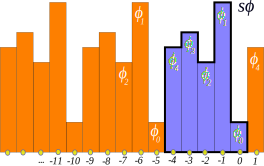
\includegraphics[width=\textwidth]{1dLatStatC_5_s0}
\\
{($\Refl_1$)}~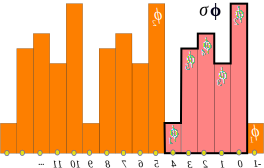
\includegraphics[width=\textwidth]{1dLatStatC_5_s1}
\\
{($\Refl_2$)}~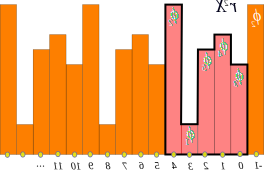
\includegraphics[width=\textwidth]{1dLatStatC_5_s2}
\\
{($\Refl_3$)}~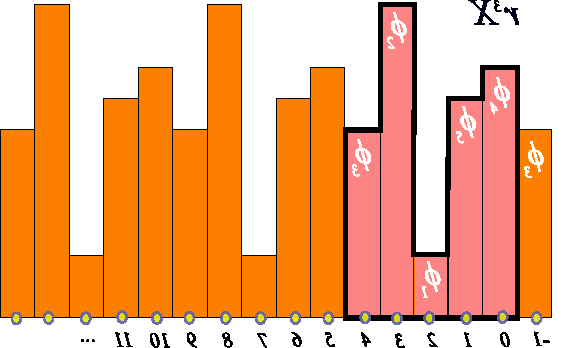
\includegraphics[width=\textwidth]{1dLatStatC_5_s3}
\\
{($\Refl_4$)}~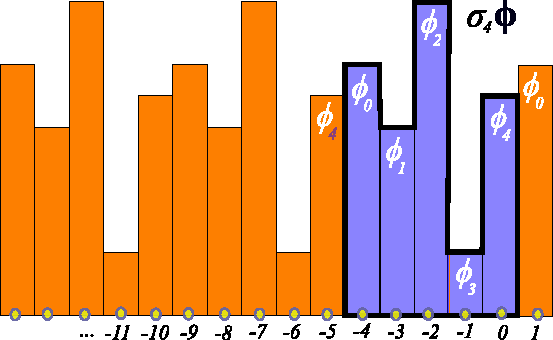
\includegraphics[width=\textwidth]{1dLatStatC_5_s4}

  \end{center} \end{minipage}
  \end{center}
%  \caption{\label{fig:1dLatStatC_5}
% (1)
{\lattstate}
% \refeq{1dLattStatC_n}
\(\Xx=\cycle{\ssp_0 \ssp_1 \ssp_2 \ssp_3 \ssp_4}\),
no reflection symmetry
\\
 translation group $H_{5}$ invariant

\Dn{\infty}-orbit is isomorphic to $\Dn{5}$ : $10$ distinct {\lattstate}s
\end{frame} %%%%%%%%%%%%%%%%%%%%%%%%%%%%%%%%%%%%%%%%%%%%%%

\begin{frame} {4 kinds of Bravais lattice states}
\begin{center}
{$(n)$}
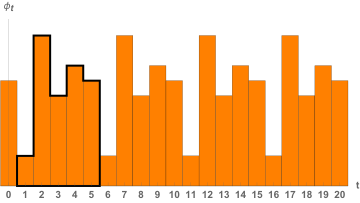
\includegraphics[width=0.40\textwidth]{HL1dLatticeStateBar1}\quad~~~
{$(o)$}
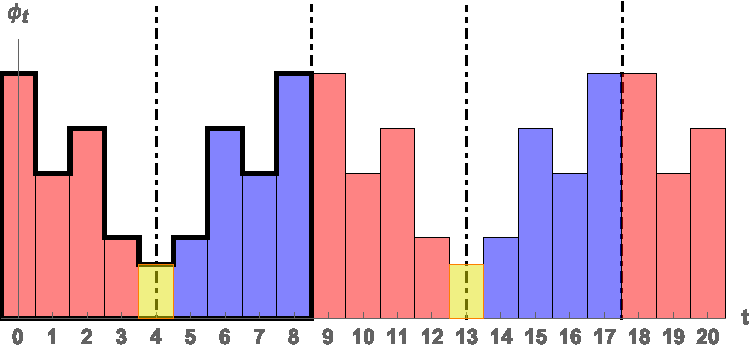
\includegraphics[width=0.40\textwidth]{HL1dLatticeStateBar2}
\\ %~~~
{$(ee)$}
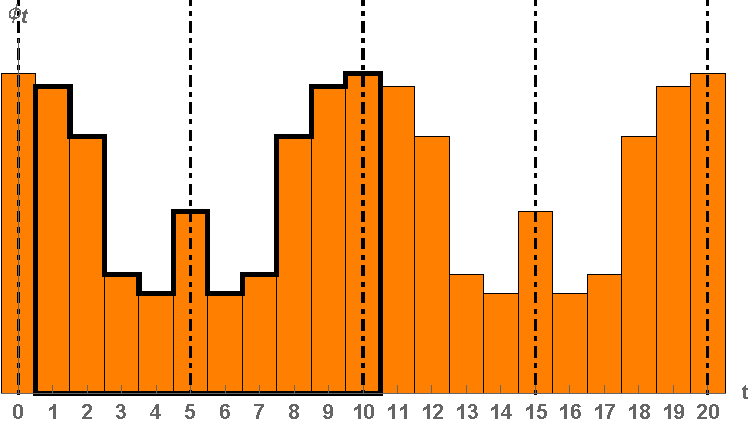
\includegraphics[width=0.40\textwidth]{HL1dLatticeStateBar4}\quad
{$(eo)$}
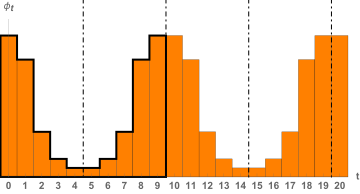
\includegraphics[width=0.40\textwidth]{HL1dLatticeStateBar3}
%\caption{\label{fig:symmLattStates}
  \end{center}

$(n)$ {\em no reflection symmetry:}
    $H_{5}$ invariant period-5 {\lattstate}

$(o)$ {\em odd period, symmetric:}
    an $H_{9,8}$ invariant period-9

$(ee)$ {\em even period, even symmetric:}
    $H_{10,0}$  invariant period-10

$(eo)$ {\em even period, odd symmetric:}
    $H_{10,9}$  invariant period-10
\end{frame} %%%%%%%%%%%%%%%%%%%%%%%%%%%%%%%%%%%%%%%%%%%%%%

\begin{frame} {example : 5-period Bravais lattice site, with reflection}
    \begin{block}{scalar \emph{field} $\ssp(x)$}
\begin{center}
            \begin{minipage}[c]{0.32\textwidth}\begin{center}
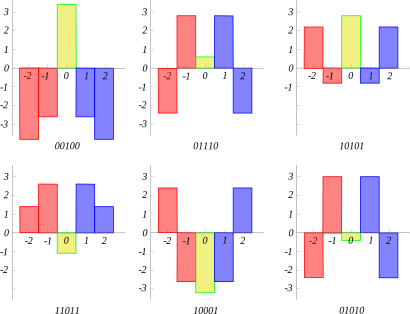
\includegraphics[width=1.00\textwidth]{PChenlatt5cyc} % from HL1dLattRefl0.svg
            \end{center}
            \end{minipage}
            \hspace{2ex}
            \begin{minipage}[c]{0.46\textwidth}
\henlatt\ period-5\\
{\lattstate}
$
\ssp_{-2} \ssp_{-1} {\ssp_0}\,\ssp_1 \ssp_2
$
\beq
\ssp_{i} = \ssp_{i+5}
    \,, \quad
\ssp_{-i} = \ssp_{i}
\,.
\ee{symmCycD5bcs}
            \end{minipage}
\end{center}
reflection symmetric; fixed lattice field ${\ssp_0}$ colored gold
%\label{fig:PChenlatt5cyc} % started with {SVW5CycHamHen}
    \end{block}
\beq
\begin{aligned}
    -S'[\ssp_{0}] + 2 \ssp_1 = -m_0 \\
\ssp_0 -S'[\ssp_{1}] +\ssp_2 = -m_1 \\
\ssp_1 -S'[\ssp_{2}] +\ssp_2 = -m_2
\end{aligned}
\ee{symmCycD5eqs} % from {HLsymmCycD5eqs}
with a 3\dmn\ {\jacobianOrb}
\bea
\jMorb &=&
\left(\begin{array}{ccc}
 {s}_0 &-2 & 0 \\
-1 & {s}_1 &-1 \\
 0 & 1 & {s}_2-1
\end{array}\right)
%\label{OrbJacobianD5} % from {HLOrbJacobianD5}
\eea
\end{frame} %%%%%%%%%%%%%%%%%%%%%%%%%%%%%%%%%%%%%%%%%%%%%%

\begin{frame}{orbit Jacobian (Hill, Hessian, ...)  matrix}
each {\lattstate} has its own
\beq
\jMorb[\Xx] =
\left(\begin{array}{cccccccc}
%\begin{pmatrix}
 {s}_{0} &-1 & 0 & 0 & \cdots & 0 & 0 &-1 \\
-1&  {s}_{1} &-1 & 0 & \cdots & 0 & 0 & 0 \\
0 &-1 &  {s}_{2} &-1 & \cdots & 0 & 0 & 0 \\
\vdots & \vdots & \vdots & \vdots & \ddots & \vdots & \vdots & \vdots \\
0 & 0 & 0 & 0 & \cdots &-1 &  {s}_{\cl{}-2} &-1 \\
-1& 0 & 0 & 0 & \cdots & 0 &-1 &  {s}_{\cl{}-1}
%\end{pmatrix}
          \end{array} \right)
\,,
\ee{jMorb1dFT} %was {jMorb1dField}, {PCJiKoKr20(8)}
{\color{orange}stretching factor} ${s}_{\zeit}= V''[\ssp_{\zeit}]$ is
\\
function of the site field $\ssp_\zeit$ for the
given \lattstate\ $\Xx$

\bigskip
  \begin{enumerate}
              \item
can compute {\color{blue}\HillDet} $\Det\jMorb$
              \item
Hill-Lindstedt-Poincar\'e : \\
all calculations should be done
on reciprocal lattice
              \item
toolbox : discrete Fourier transforms, irreps of \Dn{n}
   \end{enumerate}
\end{frame} %%%%%%%%%%%%%%%%%%%%%%%%%%%%%%%%%%%%%%%%%%%%%%

\begin{frame} {zeta functions unlike 1980's}

{\po\ theory : counting {\lattstate}s}\footfullcite{Lind96}

\begin{block}{Lind zeta function}
\beq
\zeta_{Lind}(t) =
\exp \left( \sum_{H} \;
            \frac{N_{H}}{|\Group/{H}|}t^{|\Group/H|}
      \right)
\ee{LC21Ryu17eq:1.3}
sum is over all subgroups $H$ of space group $\Group$
\\
$N_{H}$ is the number of fixed points of $H$
\\
$|\Group/{H}|$ is the number of states in $H$ orbit
\end{block}
        \begin{enumerate}
              \item
Lind zeta function counts group {\color{blue} orbits}, one per each set of equivalent
{\lattstate}s
            \end{enumerate}
\end{frame} %%%%%%%%%%%%%%%%%%%%%%%%%%%%%%%%%%%%%%%%%%%%%%

\begin{frame} {zeta functions unlike 1980's}

{\po\ theory :
\\
counting {\lattstate}s} for reflection-symmetric systems%
\footfullcite{ArtMaz65}${}^,$\footfullcite{KiLePa03}

\begin{block}{Kim-Lee-Park zeta function}
\beq
\zeta_{\Refl}(t) = \sqrt{\zeta_{top}(t^2)} \; e^{h(t)},
\ee{LC21Ryu17eq:2.1}
where $\zeta_{top}$ is the
Artin-Mazur zeta function,
and the counts of the 3 kinds of symmetric orbits are
\beq
h(t) = \sum_{m=1}^{\infty} \left\{
       N_{2m-1, 0}\,t^{2m-1}
       + \left(N_{2m,0}+N_{2m,1}\right)\,\frac{ t^{2m}}{2}
                               \right\}
\ee{LC21Ryu17eq:2.11}
\end{block}
\end{frame} %%%%%%%%%%%%%%%%%%%%%%%%%%%%%%%%%%%%%%%%%%%%%%

\begin{frame} {what we still do not understand today}
  \begin{enumerate}
              \item
solved so far only 1\dmn\ {\color{orange}spatio}{temporal} lattice,
\\
point group \Dn{1}
              \item
should all time-reversal symmetric systems be analyzed this way ?
              \item
should all dynamical systems should be solved on reciprocal lattice ?
              \item
for 2\dmn\ \spt\ chaotic field theory,
\\
still have to do this for square lattice point group \Dn{4}
              \item
then, solve the problem of turbulence \\
(Navier-Stokes, Yang-Mills, general relativity)
   \end{enumerate}
\end{frame} %%%%%%%%%%%%%%%%%%%%%%%%%%%%%%%%%%%%%%%%%%%%%%

\begin{frame} %%%%%%%%%%%%%%%%%%%%%%%%%%%%%%%%%%%%%%%%%%%%
{time reversal}
Fej{\'e}r\rf{Fejer16,RieSzo55} (1916) Fej\'er
and Riesz lemma:

every positive trigonometric polynomial can be represented by the square
of the absolute value of another trigonometric polynomial whose
coefficients are, in general, complex
\end{frame} %%%%%%%%%%%%%%%%%%%%%%%%%%%%%%%%%%%%%%%%%%%%%%

%\begin{frame} %%%%%%%%%%%%%%%%%%%%%%%%%%%%%%%%%%%%%%%%%%%%
%{symmetry}
%% In 1997 Baake, Hermisson and Pleasants\rf{BaHePl97}
%only point symmetry possible for $1-d$ lattice:
%
%mirror (inversion)
%symmetry ${\zeit}\to-{\zeit}$
%
%inversion symmetric lattice states $\ssp_{\zeit} = \ssp_{-\zeit}$
%
%infinite lattice states: with an invariant point $T\ssp_{0} = \ssp_{0}$ or
%no such $T\ssp_{\zeit} \neq \ssp_{-\zeit}$ for all $\zeit\in\integers$
%
%four such points
%\beq
%(0,0)\,\; (\frac{1}{2},0)\,\;  (0,\frac{1}{2})\,\;  (\frac{1}{2},\frac{1}{2})\,\;
%\,,
%\ee{BaHePl97(1)}
%form the discrete subgroup of ‘two-division points’ of $T^2$,
%isomorphic to $\Dn{1}\times\Dn{1}$.
%\end{frame} %%%%%%%%%%%%%%%%%%%%%%%%%%%%%%%%%%%%%%%%%%%%%%

%\begin{frame} %%%%%%%%%%%%%%%%%%%%%%%%%%%%%%%%%%%%%%%%%%%%
%{time reversal}
%\end{frame} %%%%%%%%%%%%%%%%%%%%%%%%%%%%%%%%%%%%%%%%%%%%%%
%
%\begin{frame} %%%%%%%%%%%%%%%%%%%%%%%%%%%%%%%%%%%%%%%%%%%%
%{time reversal}
%\end{frame} %%%%%%%%%%%%%%%%%%%%%%%%%%%%%%%%%%%%%%%%%%%%%%
%
%\begin{frame} %%%%%%%%%%%%%%%%%%%%%%%%%%%%%%%%%%%%%%%%%%%%
%{time reversal}
%\end{frame} %%%%%%%%%%%%%%%%%%%%%%%%%%%%%%%%%%%%%%%%%%%%%%

%%%%%%%%%%%%%%%%%%%%%%%%%%%%%%%%%%%%%%%%%%%%%%
\begin{frame}{factoring the {\jacobianOrb}}
\bea
\jMorb &=&  \Box - {\mu}^2\unit
       \,=\,
  \left(\hopMat^{-1}  - \unit \right)
  \left(\hopMat       - \unit \right)
   - {\mu}^2\unit
\,,
\label{LatLap}
\eea
where
\beq
{\mu }= \sqrt{s-2}
\,.
\ee{templattMass}
is the
Yukawa mass parameter %\refeq{catlattMass} in $d=1$ dimension.
\end{frame} %%%%%%%%%%%%%%%%%%%%%%%%%%%%%%%%%%%%%%%%%%%%%%

\begin{frame} %%%%%%%%%%%%%%%%%%%%%%%%%%%%%%%%%%%%%%%%%%%%
{XXX}
centered,
reflection (anti)symmetric difference operators
\bea
\tilde{\partial} &=&
\tilde{\hopMat}-\tilde{\hopMat}^{-1}
\,,\qquad
\tilde{\hopMat}=\hopMat^{1/2}
    \continue
 &=& - \transp{\tilde{\partial}}
\,,
\label{centeredDiffOper}
\eea
interpolate 1/2-unit spacing lattice $\tilde{\lattice}$
points between the integer lattice \lattice\ points

$\tilde{\hopMat}=\hopMat^{1/2}$ is the shift
operator on the 1/2 lattice spacing. So two applications of 1/2 lattice
shift operator give you one full lattice spacing.

\end{frame} %%%%%%%%%%%%%%%%%%%%%%%%%%%%%%%%%%%%%%%%%%%%%%

\begin{frame} %%%%%%%%%%%%%%%%%%%%%%%%%%%%%%%%%%%%%%%%%%%%
{XXX}
1/2-unit spacing lattice $\tilde{\lattice}$
points between the integer lattice \lattice\ points, with the derivatives
written as
\bea
\left(\hopMat-\unit\right)
 &=&
\tilde{\hopMat}\tilde{\partial}
     % \left(\tilde{\hopMat}-\tilde{\hopMat}^{-1}\right)
    \continue
\left(\hopMat^{-1}-\unit\right)\left(\hopMat-\unit\right)
 &=&
    - \tilde{\partial}^2
  = \Box
    %\left(\tilde{\hopMat}-\tilde{\hopMat}^{-1}\right)^2
 \label{Lat-LapSqrt}\\
\jMorb  &=& \Box - \mu^2\unit
         = \transp{\tilde{\jMorb}}\tilde{\jMorb}
%\left(
%\tilde{\partial} + \mu\unit  %\left(\tilde{\hopMat}-\tilde{\hopMat}^{-1}\right)
%\right)
%\left(
%\tilde{\partial} - \mu\unit  %\left(\tilde{\hopMat}-\tilde{\hopMat}^{-1}\right)
%\right)
    \continue
\tilde{\jMorb}
     &=& \tilde{\partial} - {\mu}\unit
    \,=\,
    \tilde{\hopMat} - \mu\unit -\tilde{\hopMat}^{-1}
    \continue
\transp{\tilde{\jMorb}}
     &=& \tilde{\partial} + {\mu}\unit
    \,=\,
    \tilde{\hopMat} + \mu\unit -\tilde{\hopMat}^{-1}
\nnu
\eea
\end{frame} %%%%%%%%%%%%%%%%%%%%%%%%%%%%%%%%%%%%%%%%%%%%%%

\begin{frame} %%%%%%%%%%%%%%%%%%%%%%%%%%%%%%%%%%%%%%%%%%%%
{XXX}
in the matrix form, the
$\jMorb=\transp{\tilde{\jMorb}}\tilde{\jMorb}$ factorization
can be checked by matrix multiplication
\bea
{\jMorb}
  &=&
\left(
\begin{array}{ccccccc}
-{s}& 0 & {1} & 0 & \dots & {1} & 0 \\
 0 &-{s}& 0 & {1} & \dots & 0 & {1} \\
 {1} & 0 &-{s}& 0 & \dots & 0 & 0 \\
 \vdots & \vdots & \vdots & \ddots & \vdots & \vdots & \vdots \\
 0 & 0 & \dots & 0 &-{s}& 0 & {1} \\
 {1} & 0 & \dots & {1} & 0 &-{s}& 0 \\
 0 & {1} & \dots & 0 & {1} & 0 &-{s}\\
\end{array}
\right)
    \continue
\tilde{\jMorb}
  &=&
\left(\begin{array}{ccccccc}
-\mu &{-1}  & 0 & 0 &\dots &0& 1\\
 1   &-\mu &{-1}& 0 &\dots &0&0 \\
 0 &  1 &-\mu &{-1}&\dots &0 & 0 \\
\vdots & \vdots &\vdots & \vdots & \ddots &\vdots &\vdots\\
 0 & 0 & \dots &\dots &\dots  &-\mu&{-1}\\
{-1}& 0 & \dots &  \dots &\dots& 1 &-\mu
        \end{array} \right)
\,,
\label{tildejMorb}  % copy of PC(1.2.11)}
\eea
where $\jMorb, \transp{\tilde{\jMorb}}, \tilde{\jMorb}$ act on the 1/2-unit
spacing lattice $\tilde{\lattice}$
\end{frame} %%%%%%%%%%%%%%%%%%%%%%%%%%%%%%%%%%%%%%%%%%%%%%

%\begin{frame} %%%%%%%%%%%%%%%%%%%%%%%%%%%%%%%%%%%%%%%%%%%%
%{XXX}
%\end{frame} %%%%%%%%%%%%%%%%%%%%%%%%%%%%%%%%%%%%%%%%%%%%%%

\begin{frame} %%%%%%%%%%%%%%%%%%%%%%%%%%%%%%%%%%%%%%%%%%%%
{"Dirac" "square root"}
the metal map
takes a temporal lattice form
\beq
\tilde{\ssp}_{\zeit+1}  -  \mu\,\tilde{\ssp}_{\zeit} - \tilde{\ssp}_{\zeit-1}
    =
-\tilde{\Ssym{\zeit}}
\,,
\ee{GoldenCatRec}
or,
in terms of a {lattice state} $\Xx$, the corresponding {symbol \brick}'
$\Mm$, and the $[\cl{}\!\times\!\cl{}]$ {\shiftOp}
$\hopMat$, % \refeq{hopMatrix},
\beq
(\tilde{\hopMat} - \mu\id - \tilde{\hopMat}^{-1})\,\tilde{\Xx} = -\tilde{\Mm}
\,,
\ee{catTempLatt}
\end{frame} %%%%%%%%%%%%%%%%%%%%%%%%%%%%%%%%%%%%%%%%%%%%%%

%\begin{frame} %%%%%%%%%%%%%%%%%%%%%%%%%%%%%%%%%%%%%%%%%%%%
%{XXX}
%\end{frame} %%%%%%%%%%%%%%%%%%%%%%%%%%%%%%%%%%%%%%%%%%%%%%
%
%\begin{frame} %%%%%%%%%%%%%%%%%%%%%%%%%%%%%%%%%%%%%%%%%%%%
%{XXX}
%\end{frame} %%%%%%%%%%%%%%%%%%%%%%%%%%%%%%%%%%%%%%%%%%%%%%

\end{document}
